\documentclass[twocolumn]{article}
\usepackage{soul}
\usepackage{amsmath}
\usepackage[utf8]{inputenc}
\usepackage[left=2cm, right=2cm, top=50]{geometry}
\usepackage{multicol}
\setlength{\columnsep}{1cm}
\usepackage{graphicx}
\usepackage{subfigure}
\title{Ellipse}
\author{Diptasri Ghosh}
\date{EE21MTECH14004}

\begin{document}

\maketitle
\textbf{\textit{Abstract} - This document contains solution of sketching loci of the given equation.}\\
\begin{center}
\textbf{\ul{Problem}}\\
Vector-2, Example-4, Question No.-7
\end{center}

\textbf{Question 7. Sketch the loci of the following equation}\\
\begin{equation}
\frac{x^2}{4} + \frac{y^2}{9} = 1
\end{equation}
\textbf{Solution :}\\
Given equation is,
\begin{equation}
\frac{x^2}{4} + \frac{y^2}{9} = 1
\end{equation}
We can write equation (2) as,
\begin{equation}
9 x^2 + 4 y^2 - 36 = 0
\end{equation}
The general equation is given as,
\begin{equation}
\textbf{x}^\top \textbf{V} \textbf{x} + 2 \textbf{u}^\top \textbf{x} + f = 0 
\end{equation}
Comparing (3) and (4) we get,
\begin{equation}
\textbf{V} = \begin{pmatrix}
9 & 0\\
0 & 4\\
\end{pmatrix} ,
\textbf{u} = \begin{pmatrix}
0\\
0\\
\end{pmatrix} , 
f = -36
\end{equation}
The vertex of ellipse is given as \textbf{c} and can be obtained from,
\begin{equation}
\textbf{c} = - \textbf{V}^-^1 \textbf{u}
\end{equation}
We know,
\begin{equation}
\textbf{V}^-^1 = \frac{1}{\begin{vmatrix}\textbf{V}\end{vmatrix}} Adj \textbf{V}
\end{equation}
Putting the values of \begin{vmatrix}\textbf{V}\end{vmatrix} and Adj \textbf{V} we get,
\begin{equation}
\textbf{V}^-^1 = \frac{1}{36} \begin{pmatrix}
4 & 0\\
0 & 9\\
\end{pmatrix}^\top 
 = \begin{pmatrix}
\dfrac{4}{36} & 0\\
0 & \dfrac{9}{36}\\
\end{pmatrix}
\end{equation}
Putting values in equation (6) we get the vertex of the ellipse,
\begin{equation}
\textbf{c} = \begin{pmatrix}
0\\
0\\
\end{pmatrix} 
\end{equation}

The length of semi major axis and semi minor axis are given by,
\begin{equation}
\sqrt{\frac{\textbf{u}^\top \textbf{V}^-^1 \textbf{u} - f}{ \lambda_1}} = 3   ,   \sqrt{\frac{\textbf{u}^\top \textbf{V}^-^1 \textbf{u} - f}{ \lambda_2}} = 2
 \end{equation}
Solving equation (10) we get,
\begin{equation}
\lambda_1 = 4   ,   \lambda_2 = 9
\end{equation}
The eccentricity of ellipse is given by,
\begin{equation}
e = \sqrt{1 - \frac{\lambda_1}{\lambda_2}}
\end{equation}
Putting the values in equation 12 we get,
\begin{equation}
e = \frac{\sqrt{5}}{3}
\end{equation}
The directrices of ellipse is given by,
\begin{equation}
c = \frac{e \textbf{u}^\top \textbf{n} \pm \sqrt{e^2 (\textbf{u}^\top n)^2 - \lambda_2 (e^2 - 1) (||\textbf{u}||^2 - \lambda_2 f)}}{\lambda_2 e (e^2 - 1)}
\end{equation}
Where
\begin{equation}
\textbf{n} = \sqrt{\lambda_2} \textbf p_1 = \begin{pmatrix}
0\\
1\\
\end{pmatrix}
\end{equation}As
\begin{equation}
 \textbf p_1 = \frac{1}{\sqrt{9}}\begin{pmatrix}
0\\
1\\
\end{pmatrix}
\end{equation}
Putting the values in equation (14) we get directrices of the ellipse,
\begin{equation}
c = \pm \frac{9}{\sqrt{5}}
\end{equation}
The foci of ellipse is given by,
\begin{equation}
\textbf{F} = \frac{c e^2 \textbf{n} - \textbf{u}}{\lambda_2}
\end{equation}
Putting the respective values in equation (18) we get,
\begin{equation}
\textbf{F} = \begin{pmatrix}
0\\
\dfrac{\sqrt{5}}{3}\\
\end{pmatrix}
\end{equation}

\begin{figure}[!ht]
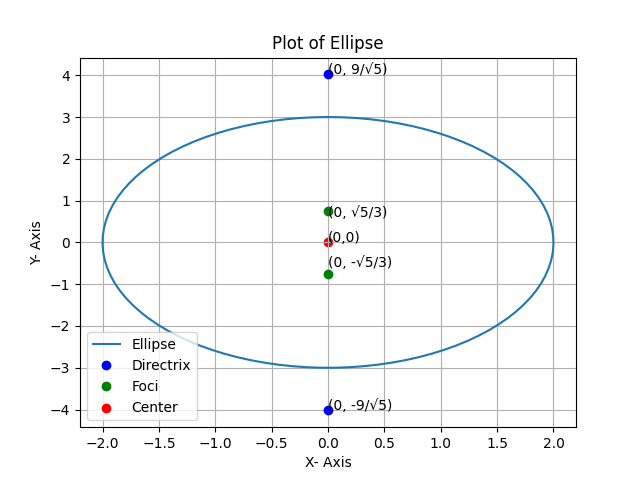
\includegraphics[width=1.1\columnwidth]{Figure_1.png}
\caption{Plot of the Ellipse with vertex \textbf{c} = \begin{pmatrix}
0\\
0\\
\end{pmatrix}  }
\label{fig}
\end{figure}
\end{document}



